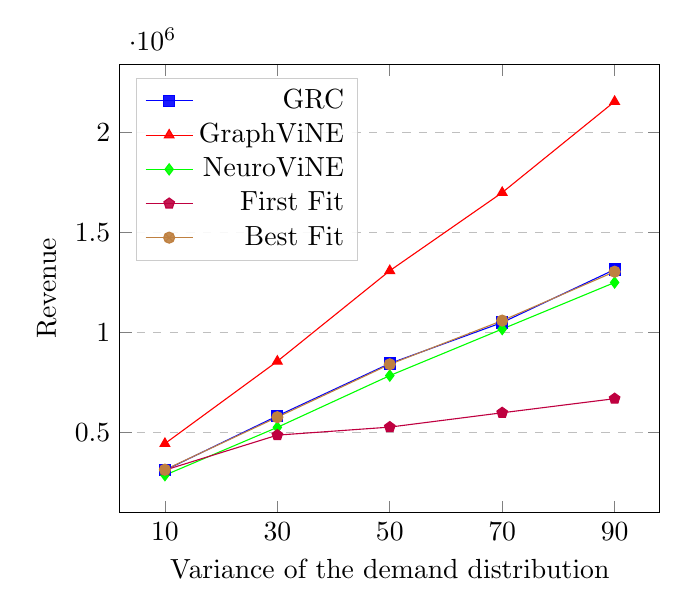
\begin{tikzpicture}
\begin{axis}[
    legend cell align={right},
    legend style={fill opacity=0.9, draw opacity=1, text opacity=1, draw=white!80!black},
    xlabel={Variance of the demand distribution},
    ylabel={Revenue},
    % xmin=0, xmax=100,
    % ymin=0, ymax=1,
    xtick={0,10,30,50,70,90, 100},
    % ytick={0,100,200,300,400,500},
    legend pos=north west,
    ymajorgrids=true,
    grid style=dashed,
]

\addplot[
    color=blue,
    mark=square*,
    ]
    coordinates {
(10,310278)
(30,581754)
(50,844107)
(70,1048861)
(90,1313781)
    };
\addlegendentry{GRC}

\addplot[
    color=red,
    mark=triangle*,
    ]
    coordinates {
(10,443410)
(30,854997)
(50,1307757)
(70,1698651)
(90,2153743)
    };
\addlegendentry{GraphViNE}

\addplot[
    color=green,
    mark=diamond*,
    ]
    coordinates {
(10,285606)
(30,524704)
(50,783399)
(70,1016251)
(90,1248881)
    };
\addlegendentry{NeuroViNE}

\addplot[
    color=purple,
    mark=pentagon*,
    ]
    coordinates {
(10,310806)
(30,485756)
(50,525896)
(70,597567)
(90,668085)
    };
\addlegendentry{First Fit}

\addplot[
    color=brown,
    mark=otimes*,
    ]
    coordinates {
(10,312989)
(30,575444)
(50,839820)
(70,1058408)
(90,1302955)
    };
\addlegendentry{Best Fit}





\end{axis}
\end{tikzpicture}